\adparagraph{nDCG}
Figure \ref{fig:ndcg} shows the nDCG score for BC, \MC, SF, and Avg. For nDCG a higher score is better as covered in Section \ref{sec:methodology_ndcg}.\note{this is not explicitly covered in that section}
All methods see a sharp drop off in the quality of their recommendations as the group sizes increase.
As shown in Table \ref{tbl:ndcg}, BC drops the most in the jump from 4 to 8 group members, however it also have the best results, and outperforms all other methods across all group sizes.
\MC is second best by only a few percentage points and follows the same trend and quickly plateaus in score.
One outlying case SF starts out close to Avg for a group size of four, but retains a higher score and is closer to BC and \MC as the size increases.
Avg is the worst performing overall.

\begin{figure}[H]
	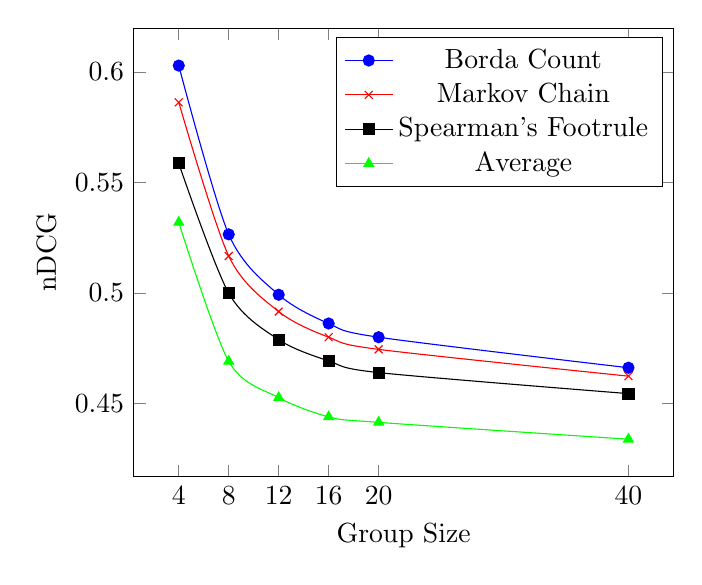
\begin{tikzpicture}
	\begin{axis}[
	xlabel=Group Size,
	ylabel=nDCG,
	xtick = {4,8,12,16,20,40}]
	\addplot[smooth,mark=*,blue] plot coordinates {
		(4,0.6028)
		(8,0.5265)
		(12,0.4992)
		(16,0.4862)
		(20,0.48)
		(40,0.4662)
	};
	\addlegendentry{Borda Count}

	\addplot[smooth,color=red,mark=x] plot coordinates {
		(4,0.5862)
		(8,0.5167)
		(12,0.4916)
		(16,0.48)
		(20,0.4745)
		(40,0.4624)
	};
	\addlegendentry{Markov Chain}
	
	\addplot[smooth,color=black,mark=square*] plot coordinates {
		(4,0.5586)
		(8,0.4999)
		(12,0.4789)
		(16,0.4693)
		(20,0.464)
		(40,0.4545)
	};
	\addlegendentry{Spearman's Footrule}
	
	\addplot[smooth,color=green,mark=triangle*] plot coordinates {
		(4,0.5319)
		(8,0.4691)
		(12,0.4527)
		(16,0.444)
		(20,0.4415)
		(40,0.4339)
	};
	\addlegendentry{Average}
	
	\end{axis}
	\end{tikzpicture}
	\caption{Results for nDCG test}\label{fig:ndcg}
\end{figure}

\begin{table}[H]
	\centering
	\begin{tabular}{|l|lllll|}\hline
		& 4 to 8 & 8 to 12 & 12 to 16 & 16 to 20 & 20 to 40 \\\hline
		BC 	& 12.66	& 5.19	& 2.6	& 1.28	& 2.88 \\
		MC  & 11.86	& 4.86	& 2.36	& 1.15	& 2.55 \\
		SF  & 10.51	& 4.20	& 2.00	& 1.13	& 2.05 \\
		Avg	& 11.81	& 3.50 	& 1.92	& 0.56	& 1.72 \\ \hline
	\end{tabular}
	\caption{Percentage decrease between the groups for nDCG}
	\label{tbl:ndcg}
\end{table}